% NC: I'm not sure that this is necessary for this paper. It's much more linear that the previous one. You could save for the supp mat or your thesis 
%To test whether mammals display a significant change in disparity after the K-Pg boundary we use the following protocol (note that each step is explained in detail below this section; Fig.~\ref{fig_method}.
%\begin{enumerate}
%\item{Data: we used the cladistic morphological matrices and the Total Evidence tip-dated trees published in \citep{Slater2012MEE} and \citep{beckancient2014}.} \\
%\item{Estimating ancestral character states: we used the \citep{Yang01121995} re-rooting method to estimate the states of each characters in the cladistic morphological matrices at each node and created the reconstructed morphological matrix containing observed morphological characters data for tips in the tree and estimated morphological characters states for nodes.}\\
%\item{Calculating the cladisto-space: using the reconstructed morphological matrix we defined the cladisto-space by using a principal components ordination of the Gower distance matrix \citep{Gower71} representing the $n$ finite dimensional space that encompasses the total cladistic morphological variation of the taxa present in the analysis.} \\
%\item{Time slicing: we then separated the cladisto-space into subdivisions containing only the edges (nodes or/and tips) present every 5 million years from present (hereafter called "time-slices").} \\
%\item{Disparity through time: we then calculate the phylogenetic diversity as the number of edges present at each time-slice as well as the cladistic morphological disparity defined as the spread of the edges in the cladisto-space at each time-slice (distance from cladisto-space centroid \citep{finlay2015morphological}.} \\
%\item{Null model testing: finally, we compared the observed disparity to the expected disparity under two different null models: (1) the first one being a completely stochastic model where disparity is random at each point in time.; and (2) the second one being a $Mk_n$ model (as a proxy for Brownian evolution) where disparity increase is constant through time.} \\
%\end{enumerate}

%\begin{figure}[!htbp]
%\centering
%    \includegraphics[keepaspectratio=true]{Figures/MEthod_outline.pdf}
%\caption{General method outline. The grey section represents the Total Evidence data and tip dated trees from two published studies \citep{Slater2012MEE,beckancient2014}. \textbf{A}: We then estimated the ancestral characters states from the observed morphological matrices from both studies. we then calculated the distance matrix using the Gower distance \citep{Gower71} and performed a ordination of the distance matrix to create the cladisto-space. Finally, we divided the cladisto-space matrix using the Time slicing method to measure the changes in morphological disparity through time. \textbf{B}: we then generated two sets of a hundred simulated "null" matrices under two null models, the random matrix: a fully stochastic matrix; and the $Mk_n$ matrix: a matrix simulated under the $Mk_n$ model. We then applied the same procedure as for \textit{A} (ordinated distance matrix and time slicing) to calculate the disparity through time expected for purely random data and for a constant evolution model. Finally we compared our simulated disparity through time to our observed disparity through time to estimate if mammals displayed a significant increase in disparity after the K-Pg boundary.}
%\label{fig_method}
%\end{figure}


%We tested the effect of this assumption against another model where each missing character is treated as ``?'' character. In this second model, the missing data (NA) is treated as a new character ``?'' and the state of the character at the node can then be 0, 1 or ``?''. This method is more conservative because it does not make the assumption that the unobserved characters for taxa with missing data is obligatory one of the states observed for that character. However, simulations show that the first method (treating missing data as multi-state characters) leads to less false positive ancestral state reconstruction than the second (treating missing data as ``?'' character). %link to supp % TG: I'm not sure if that's important here. Nobody cares about this I assume and it has not much to do here. Maybe in the thesis?

%We preferred Maximum Likelihood methods to Bayesian methods because both methods have been shown to produce similar results \citep{royer-carenzichoosing2013} but Maximum Likelihood methods are several orders of magnitude faster than Bayesian ones (total analysis time $\sim$@1.2 CPU year). 

 %steps described in detail below: (1) calculating the distance matrix and (2) the ordination of the distance matrix. % TG: note however that Graeme seems to say the ordination part is useless in cladistic data case. I'm not sure if he's right and I didn't did any testing but his argument make sense: ordination is to summarize the data which is useful with continuous data but less with discrete characters. However statistically I'm not sure how the disparity calculation will work since it is traditionally done on the eigen vectors (PC scores) which is just a "scaling" of the values using the covariance matrix. Therefore, if I want to use just the distance matrix, I'm afraid I'll have to find a complex way to add the covariance to the variance without using the eigen values (that make life easier in this case). Also that'll lead to problems with negative covariance (see Cailliez correction below).

 %Also one practical reason to not use the products of ranges or variances, when using the full cladisto-space (i.e. without excluding the last dimensions), is that the disparity values will tend towards 0 since the variance or ranges on the last axis are usually really close to 0. % TG: or maybe that's useless. We're already making the point that's it statistically incorrect. No need to add that it also doesn't work in practice, no?

Unfortunately, including the covariance terms in the sum and products of ranges and variances is not straightforward and comes with properties specific to the number of dimensions involved \citep{Jackson,DonohueDim}.
% NC: What do you mean it "comes with properties". Be clear.
%One potential solution is to measure the hyper-dimensional volume \citep{Wills1994,DonohueDim} but this volume based on the eigenvalue 
% NC: eigenvalue or eigenvalues? Of the distance matrix?
%cannot be calculated through time (unless one recalculates the cladisto-space at each time point).
% NC: Why mention all this if you're not going to use hypervolumes?

% TG: not sure if this figure is useful and pretty sure that if it is, it should be improved!
%\begin{figure}[!htbp]
%\centering
%    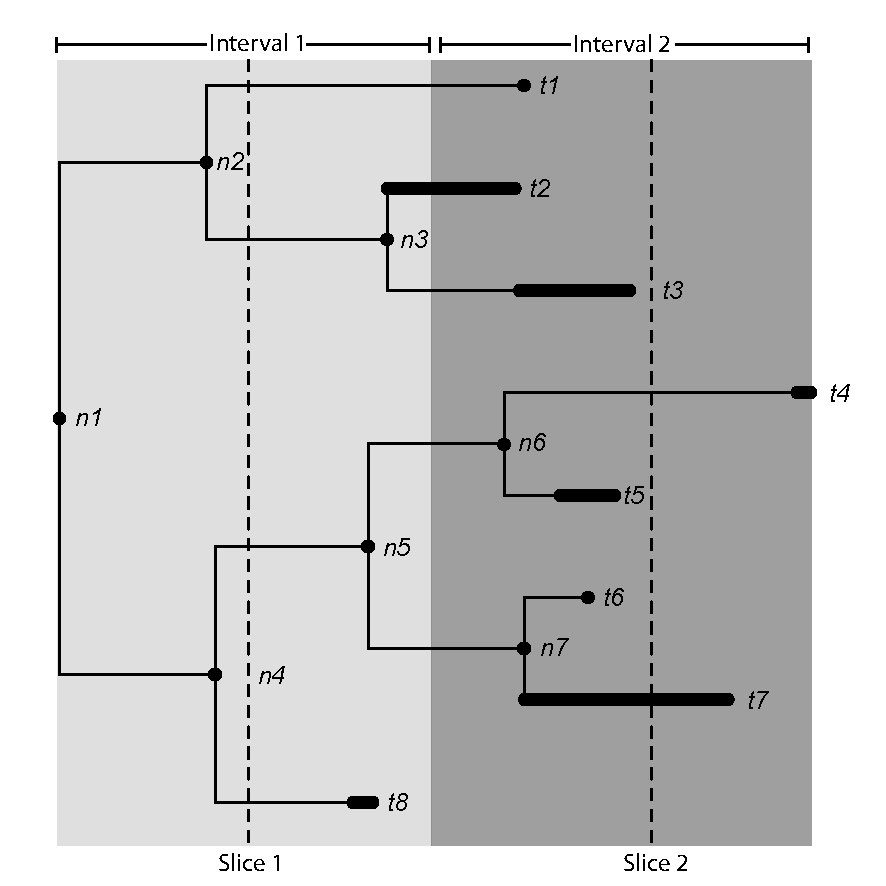
\includegraphics[keepaspectratio=true]{Figures/Slicing.pdf}
%\caption{Differences in slicing method and intervals. Solid lines represent the First and Last Appearance Datum span. Interval 1 contains the following elements within the global character-space: taxa t2 and t8 and nodes n1, n2, n3, n4 and n5. Interval 2 contains the following elements within the global character-space: taxa t1, t2, t3, t4, t5, t6 and t7 and nodes n6 and n7. Slice 1 contains the following elements within the global character-space under the proximity model (constant evolution assumption): nodes n2 and n4. Slice 2 contains the following elements within the global character-space under the proximity model (constant evolution assumption): taxa t4 and t7.}
%\label{fig_slicing}
%\end{figure}
% NC: I don't think this figure helps as it is at present. For the thesis it might be nice to have a super simple one just with dots or crosses on the branches and tips where your slice overlaps.
